\chapter{Úvod}
Úlohou projektu bolo navrhnúť, implementovať a otestovať \textbf{IRC} bota so \textbf{SYSLOG} zaznamenávaním. V~nasledujúcich kapitolách sú opísané dôležité časti projektu.

V~kapitole 2 prebieha úvodom do problematiky, ozrejmením nevyhnutých pojmov. Kapitola 3 sa zaoberá návrhom programu. V~kapitole 4 je opísaná jeho samotná implementácia. Kapitola 5 obsahuje informácie o~priebehu ladenia a testovania. Kapitola 6 poskytuje prehľad nad používaním programu. V~kapitole 7 sú uvedené základné informácie o~programe. Posledná kapitola zhrňuje získané vedomosti a skúsenosti z~projektu.
 

\chapter{Súhrn pojmov}
Táto kapitola obsahuje vysvetlenie jednotlivých pojmov súvisiacich s~projektom.

\section{IRC}
Protokol \textbf{IRC} (Internet Relay Chat) je textovo založený aplikačný protokol určený na okamžitú textovú komunikáciu. Používa \textbf{TCP} a voliteľne aj \textbf{TLS}. Najznámejší port pre IRC je \textbf{6667}. Za jeho tvorcu je považovaný Jarkko Oikarinen. Protokol je opísaný v~dokumente \textbf{RFC 1459} \cite{rfc1459}. Primárne je určený na komunikáciu skupín v~miestnostiach tzv. kanáloch ale umožňuje aj komunikáciou jedného používateľa s~druhým pomocou súkromných správ.

IRC je založený na klient--server architektúre. IRC klient je program, pomocou ktorého sa používateľ pripája k~IRC serveru a kanálu a komunikuje s~ostatnými pripojenými používateľmi. Medzi najznámejšie klienty patrí mIRC, HexChat, ChatZilla. IRC klienti sa pripájajú na IRC servery. Jediná povolená sieťová konfigurácia je spanning tree. IRC servery sa môžu pripojiť na iné IRC servery a týmto spôsobom rozšírujú IRC sieť. IRC servery zväčša nevyžadujú prihlásenie používateľov, ale je požadované nastavenie prezývky (nickname) pred pripojením na kanál. Prezývka nesmie mať viac ako 9 znakov.

\begin{figure}[h]
	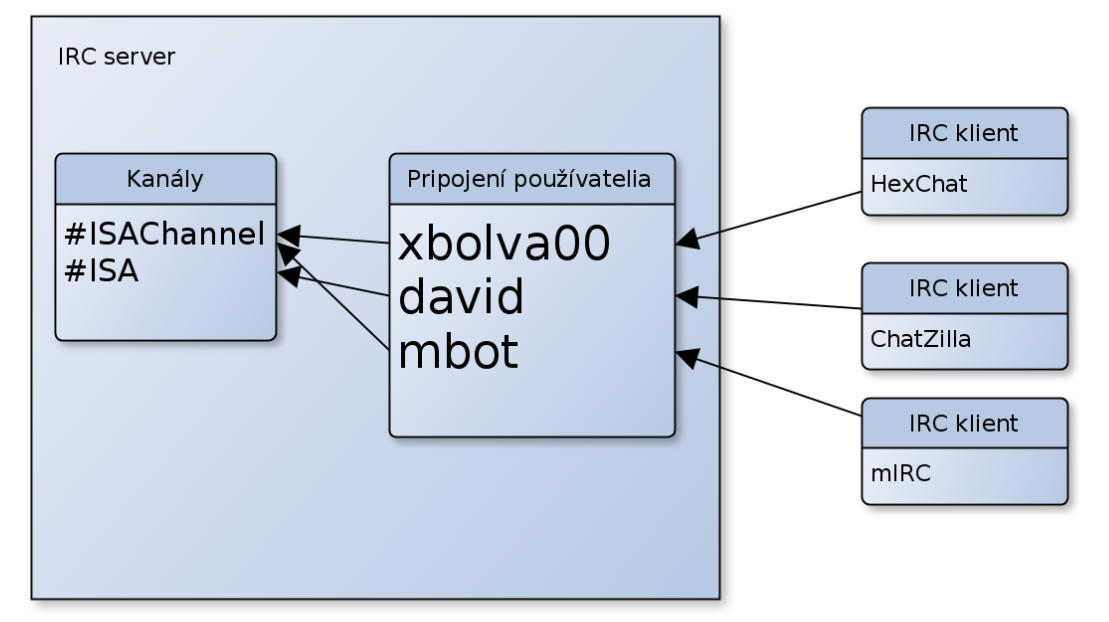
\includegraphics[width=\textwidth]{irc_arch}
	\caption{IRC klient server architektúra}
\end{figure}

\newpage

Existujú rôzne typy používateľov IRC. Zakladateľ kanálu je používateľ, ktorý založil kanál. Na danom kanáli ma najvyššie práva a kompletnú správu kanálu. Operátor kanálu má čiastočné práva na správu kanálu získané od zakladateľa kanálu. Ostatní používatelia nemajú žiadne práva na akúkoľvek správu kanálu.

Kanály sú pomenované skupiny jedného alebo viac klientov. Všetci v~tejto skupine prijímajú správy pre tento kanál. Kanál sa zakladá po pripojení prvého používateľa a zaniká po odchode posledného. Názvy kanálov začínajú znakmi @ alebo \&, nesmú obsahovať znaky medzery a čiarky a ich maximálna dĺžka je 200 znakov.

\subsection{IRC správy}
Servery a klienti si odosielajú správy medzi sebou. Ak správa obsahuje platný príkaz, klient očakáva odpoveď. Každá IRC správa obsahuje tri hlavné časti. Prvou je voliteľný \textbf{prefix}, druhou je \textbf{príkaz} a tretia časť obsahuje \textbf{parametre príkazu}. Časti su oddelené jednou alebo viacerými medzerami. Správy sú zakončené pomocou sekvencie znakov \textbf{CLRF} (\uv{\textbackslash{r}\textbackslash{n}}). V~sekcii 2.3.1 v~RFC 1459 \cite{rfc1459} je uvedený formát správy v~BNF. IRC správa nesmie presiahnuť dĺžku 512 znakov (vrátane CLRF).

\newpage

\subsection{IRC príkazy}

Významné IRC príkazy sú:
\begin{itemize}
	\item \textbf{PRIVMSG} <msgtarget> <message>
	\begin{framed}
		odoslanie správy (<message>) na cieľ (<msgtarget>) (používateľ alebo kanál).
	\end{framed}

	\item \textbf{NOTICE} <msgtarget> <message>
	\begin{framed}
		odoslanie správy (<message>) na cieľ (<msgtarget>) (používateľ alebo kanál)
		
		automatické odpovede nesmú byť odosielané ako odpovede na NOTICE správy
	\end{framed}

	\item \textbf{JOIN} <channels> [<keys>]
	\begin{framed} 
		pripojenie ku kanálom (<channels>)
	\end{framed}
	
	\item \textbf{PART} <channels> [<message>] 
	\begin{framed} 
		odchod z~kanálov <channels>
	\end{framed}
	
	\item \textbf{KICK} <channel> <client> [<message>]
	\begin{framed} 
		odstránenie klienta (<client>) z~kanálu (<channel>)
	\end{framed}

	\item \textbf{NICK} <nickname> [<hopcount>]
	\begin{framed} 
		zmena prezývky klienta
	\end{framed}

\newpage
	
	\item \textbf{PING} <server1> [<server2>] 
	\begin{framed} 
		testovanie pripojenia k~serveru
	\end{framed}
	
	\item \textbf{PONG} <server1> [<server2>] 
	\begin{framed} 
		odpoveď na PING príkaz
	\end{framed}
	
	\item \textbf{QUIT} [<message>] 
	\begin{framed} 
		odpojenie klienta od servera
	\end{framed}
\end{itemize}

\section{SYSLOG}
\textbf{Syslog} je protokol slúžiaci na zaznamenávanie správ. Protokol je opísaný v~dokumente \textbf{RFC 3164} \cite{rfc3164}. Typ architektúry je klient--server. Syslog správy je možné posielať cez \textbf{UDP aj TCP} protokoly. UDP port pridelený Syslogu je \textbf{514}, u~TCP je to \textbf{6514}. Správy sa odkazujú na zariadenia (\textbf{Facility}), ako napr. auth, deamon, local0, atď. Správam sú tiež pridelené úrovne závažnosti (\textbf{Severity})-- Emergency, Alert, Critical, Informational, atď.

\subsection{Syslog správy}
Celý formát Syslog správy sa skladá z~troch častí - \textbf{PRI}, \textbf{HEADER} a \textbf{MSG}. Celková dĺžka paketu nesmie presiahnuť 1024 bytov. \textbf{PRI} časť sa skladá z~3 až 5 znakov. Začína znakom \uv{<}, nasledovaným číslom a znakom \uv{>}. Číslo udáva prioritu, ktorá reprezentuje zariadenie/subsystém a mieru závažnosti. Túto hodnotu získame nasledovne:
\begin{framed} 
PRI = Facility * 8 + Severity
\end{framed}
Druhá časť, \textbf{HEADER}, obsahuje položku \textbf{TIMESTAMP}, kde sa nachádza dátum, čas, názov hostiteľa. Položky su oddelené medzerou. Dátum a čas je uvedený vo formáte \uv{\textbf{Mmm dd hh:mm:ss}}, kde Mmm je skrátený anglický názov mesiaca (Jan, Feb, atď.). Nasleduje \textbf{HOSTNAME} -- ak je adresa hostiteľa neznáma, použije sa IP adresa odosielateľa. Nasleduje tretia časť zvaná \textbf{MSG}, ktorá siaha až do konca paketu. Na začiatku nájdeme \textbf{TAG}, t.j. informácia o~procese/programe, ktorý správu odoslal na Syslog server. Maximálna dĺžka tohto identifikátora je 32 znakov. Prvý nealfanumerický znak značí koniec identifikátora a začiatok druhej časti, tzv. \textbf{CONTENT}, ktorý obsahuje text správy.

\begin{framed}
<PRI>TIMESTAMP HOSTNAME TAG CONTENT
\end{framed}
	
\chapter{Návrh programu}

Nasledujúci obrázok popisuje návrh samotného programu, jeho jednotlivé časti/moduly.

\begin{figure}[h]
	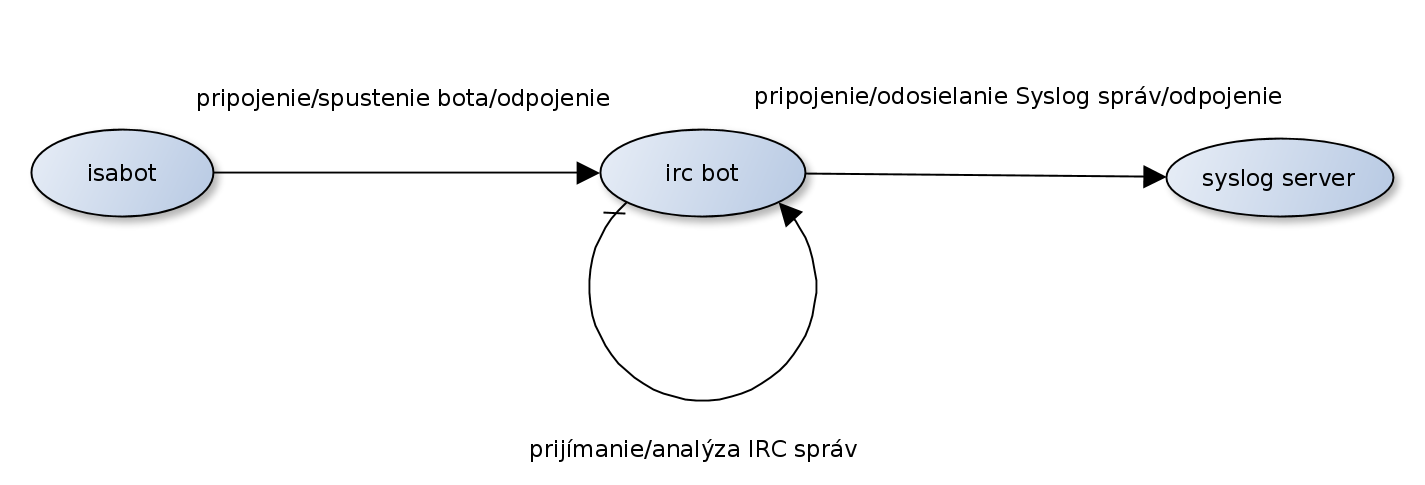
\includegraphics[width=\textwidth]{navrh}
	\caption{Návrh programu}
\end{figure}

Vstupný bod program je isabot, ktorý spracuje a skontroluje argumenty z~terminálu. Ak nedôjde k~chybe v~tejto fáze, isabot požiada IRC bota o~pripojenie k~IRC serveru na daný kanál/kanály. Následne sa spustí samotné prijímanie správ a ich analýza. IRC bot sa pripojí na Syslog server, kde sa budú zaznamenávať IRC správy, ktoré obsahujú zadané kľúčové slová. V~prípade špecifického textu v~správe spúšťa IRC bot svoje dve funkcie pre výpis dátumu alebo odoslanie správy. Po prijatí SIGINT signálu isabot požiada IRC bota o~odpojenie od IRC aj Syslog servera a program sa ukončí.

\chapter{Implementácia programu}

Program je napísaný v~jazyku C++, v~štandarde \textbf{C++14}. Sieťová komunikácia je implementovaná pomocou \textbf{BSD} schránok. Program podporuje \textbf{IPv4} aj \textbf{IPv6} adresy. IPv6 adresa musí byť zadaná spolu s portom, keďže oddelovač adresy a portu je znak dvojbodky a nebolo by možné pre program zistiť, či dvojbodka je súčasť adresy, alebo je oddelovačom adresy od portu. Jednotlivé logické celky su umiestnené v~triedach. 

V~súbore isabot.cc je samotný vstup programu (funkcia main). V~nej sa volá funkcia \textbf{parse\_args}, ktorá spracováva vstup z~terminálu. V~prípade chyby je vyhodená výnimka \textbf{argument\_exception} s~popisom chyby, ktorý sa vypíše na štandardný chybový výstup a program sa ukončí s~návratovým kódom 1. Následne sa nastavuje vlastná reakcia na prijatie SIGINT signálu -- po prijatí tohto signálu IRC bot sa odpojí od IRC servera a program sa ukončí. Ak sa nastavenie vlastnej reakcie na signál SIGINT nepodarí, program sa ukončí s~návratovým kódom 3. IRC bot sa pripája k~IRC serveru a spúšťa svoj beh. V~prípade chyby v~sieťovej komunikácii (napr. nepodarí sa pripojiť k~IRC serveru) je vyhodená výnimka \textbf{network\_exception} s~popisom chyby, ktorý sa vypíše na štandardný chybový výstup a program sa ukončí s~návratovým kódom 2. Ak nedôjde k~žiadnym chybám počas behu programu, program sa ukončí s~návratovým kódom 0 po prijatí SIGINT signálu.

Súbor irc\_bot.cc obsahuje triedu \textbf{irc\_bot}, ktorá zapuzdruje kód súvisiaci s~IRC botom. Nachádzajú sa tu funkcie pre pripojenie/odpojenie sa k~IRC serveru, spustenie samotného behu IRC bota, kde sa prijímajú a analyzujú IRC správy.

Program načítava znaku po znaku pomocou funkcie recv z~IRC servera a pripája znaky do reťazca. Po prijatí znaku sa následne kontroluje, či tento reťazec je zakončený sekvenciou znakov CLRF. Ak áno, vytvorí sa objekt triedy \textbf{irc\_command} (implementovaná v~irc\_command.cc), ktorá ponúka metódy na zistenie typu príkazu a analýzu a detekciu častí IRC správ.

Pripojenie, odosielanie správ a odpojenie od Syslog servera je implementované v~triede \textbf{syslog\_server}, implementované v~súbore syslog\_server.cc. Ďalej je tu metóda na získanie časového razítka (timestamp), ktoré je súčasťou Syslog správy. Poslednou metódou v~tejto triede je funkcia na získanie IP adresy odosielateľa, ktorá je taktiež súčasť Syslog správy.

Pomocné funkcie, ktoré sa používajú v~rôznych miestach programu, sú implementované v~súbore utils.cc. Je tu funkcia na prevod reťazca na pole (vektor) slov, slová sú v~reťazci oddelené medzerami. Ďalej je tu funkcia na prevod pola (vektoru) reťazcov na jeden reťazec, medzi jednotlivé reťazce je pridaný znak čiarky. 

\newpage

\subsection{Pripojenie ku IRC kanálu}
Po pripojení k~IRC serveru sa odošle nasledovná sekvencia IRC príkazov. Každý príkaz je zakončený sekvenciou znakov CLRF.
\begin{framed}
	NICK xbolva00
	
	USER xbolva00 xbolva00 xbolva00 :xbolva00
	
	JOIN kanál{, kanál}
\end{framed}

Ak dôjde k~chybe počas tejto fázy (ban na IRC kanáli, kanál je neplatný, atď), program sa ukončí a o~vyskytnutej chybe je používateľ informovaný správou na štandardný chybový výstup.

\newpage

\subsection{Analýza IRC správ}

Nasledujúci algoritmus popisuje implementáciu analýzy IRC správ po jej prijatí z~IRC servera.


\SetKwInput{KwData}{Vstup}
\SetKwInput{KwResult}{Výstup}

\begin{algorithm}
	\KwData{IRC správa zakončená CLRF}
	\KwResult{Spracovaná IRC správa}
	\If{príkaz PING}{
		pošli príkaz PONG s~parametrom označujúcim server z~PING správy
	} 
	\If{príkaz PRIVSMG alebo NOTICE}{
		zisti prezývku, kanál, text správy
		
		\If{kľúčové slovo sa nachádza v~slovách textu správy}{
			vytvor a odošli správu na Syslog server
		}
	
		\If{príkaz PRIVSMG a správa obsahuje kanál}{
			\If{text správy je \uv{?today}}{
				pošli príkaz PRIVMSG na IRC server, text správy je aktuálny dátum na zariadení kde beží IRC bot vo formáte \uv{dd.mm.yyyy}
			}
		
			\If{text správy je vo formáte \uv{?msg prezývka:správa}}{
				\eIf{je používateľ s~danou prezývkou pripojený na kanáli}{
					pošli príkaz PRIVMSG na IRC server, text správy je vo formáte \uv{prezývka:správa}
				} {
				    ulož si správu do interného pola (vektora) správ na neskoršie odoslanie v~prípade, že sa daný používateľ pripojený na kanál
				}
			}
		}
	}

	\If{príkaz JOIN}{
		zisti prezývku, kanál, text správy
		
		zmen stav používateľa v~interných záznamoch na stav pripojený
		
		ak existujú čakajúce správy pre tohto používateľa, odošli ich
	} 

	
	\caption{Algoritmus analýzy IRC správ}

\end{algorithm}

\newpage

\begin{algorithm}
	\KwData{IRC správa zakončená CLRF}
	\KwResult{Spracovaná IRC správa}
	\If{príkaz QUIT}{
		zisti prezývku, v~interný štruktúrach pre každý kanál nájdi tohto používateľa a zmeň jeho stav na nepripojený
	} 
	
	\If{príkaz PART}{
		zisti prezývku, kanál
		
		v~interný štruktúrach pre daný kanál/kanáli nájdi tohto používateľa a zmeň jeho stav na nepripojený
	} 

	\If{príkaz KICK}{
		zisti prezývku vyhodeného používateľa, kanál
		
		\eIf{prezývka sa zhoduje s~\uv{xbolva00}}{
			vypíš informáciu o~vyhodení IRC bota z~kanálu, ukonči program
		} {
			v~interných štruktúrach pre daný kanál/kanáli nájdi tohto používateľa a zmeň jeho stav na nepripojený
		}
	}

	\If{príkaz NICK}{
		zisti starú a novú prezývku
		
		v~interných štruktúrach zmeň starú prezývku používateľa na novú
		
		ak existujú čakajúce správy pre novú prezývku používateľa, odošli ich
	} 

	\If{príkaz RPL\_NAMREPLY (353)}{
		zisti zoznam prezývok aktuálne pripojených používateľov, kanál
		
		v~interných štruktúrach pre daný kanál nájdi týchto používateľov a zmeň ich stav na pripojený
	}
	
	\If{chyba obmedzujúca beh IRC bota}{
		zisti text správy informujúci o~chybe
		
		vypíš text o~chybe, ukonči program
	}

	\caption{Algoritmus analýzy IRC správ - pokračovanie}
		
\end{algorithm}

\newpage 

Chyby obmedzujúca beh IRC bota sú napríklad:
\begin{itemize}
	\item vyhodenie z~kanála (KICK)
	\item neplatný kanál -- ERR\_NOSUCHCHANNEL (403)
	\item pripojenie na príliš veľa kanálov -- ERR\_TOOMANYCHANNELS (403)
	\item nemožnosť odosielania správ na kanál -- ERR\_CANNOTSENDTOCHAN (404)
	\item pripojenie sa na príliš veľa kanálov -- ERR\_TOOMANYCHANNELS (405)
	\item prezývku IRC bota (\uv{xbolva00}) už niekto používa na danom kanáli -- ERR\_NICKNAMEINUSE (433)
	\item kanál je plný -- ERR\_CHANNELISFULL (471)
	\item kanál len na pozvanie -- ERR\_INVITEONLYCHAN (473)
	\item ban na kanáli -- ERR\_BANNEDFROMCHAN (474)
\end{itemize}


\subsection{Funkcie IRC bota}
Ak sa v~texte správy s~príkazom \textbf{PRIVMSG} nachádza text \uv{\textbf{?today}}, IRC bot odošle aktuálny čas vo formáte \uv{\textbf{dd.mm.yyyy}} na daný kanál získaný pomocou funkcie std::localtime. Ďalej, ak text správy sa zhoduje s~formátom \uv{\textbf{?msg prezývka:správa}}, program zistí, či používateľ s~touto prezývkou je pripojený na danom kanáli. Ak áno, pošle mu správu na daný kanál. Ak nie, správu si uloží do asociatívneho kontajnera std::map\footnote{\url{http://en.cppreference.com/w/cpp/container/map}}, kde kľúčom je reťazec (std::string\footnote{\url{http://en.cppreference.com/w/cpp/string/basic_string}}) označujúci prezývku používateľa a hodnotou je vektor reťazcov (std::vector<std::string>\footnote{\url{http://en.cppreference.com/w/cpp/container/vector}}), ktoré reprezentujú jednotlivé čakajúce správy na odoslanie. Ďalej existuje nadradený asociatívny kontajner, kde kľúčom je názov kanála a hodnotou je vyššie spomínané asociatívny kontajner s~používateľmi (na danom kanáli) a čakajúcimi správami na odoslanie pre týchto používateľov. Následne sa čaká, kým sa daný používateľ znova pripojí na kanál. Pri porovnávaní prezývok nezáleží na veľkosti písmen. Sledovanie pripojených používateľov prebieha nasledovne: po pripojení IRC bota mu IRC server zašle správu \textbf{RPL\_NAMREPLY} (353) so zoznamom aktívnych používateľov na danom kanáli a pomocou tohto zoznamu si bot zostaví prvotný zoznam používateľov a nastaví ich stav na pripojený. Následne IRC bot sleduje príkaz \textbf{JOIN}, po pripojení používateľa sa záznam pridá do tohto zoznamu so stavom používateľa ako pripojený. IRC bot sleduje príkazy \textbf{KICK}, \textbf{PART}, \textbf{QUIT}. Pri príkaze KICK sa získa prezývka vyhodeného používateľa, ak je to prezývka IRC bota (\uv{xbolva00}), program sa ukončí, lebo došlo k~obmedzeniu jeho funkcionality na danom kanáli. V~ostatných prípadoch sa v~zozname používateľov nájde daný používateľ s~touto prezývkou a jeho stav sa zmení na nepripojený. V~prípade príkazu PART si v~zozname používateľov u~kanálu, z~ktorého používateľ odišiel, nájdeme tohto používateľa a taktiež zmeníme jeho stav na nepripojený. U~príkazu QUIT sa zmení stav používateľa na nepripojený v~zozname používateľov pre každý sledovaný kanál. IRC bot sleduje aj zmenu prezývok na kanáli pomocou príkazu \textbf{NICK}, ak dôjde k~zmene, táto zmena je aplikovaná aj v~zoznamoch používateľov, ktoré si spravuje IRC bot. V~prípade, že má IRC bot uložené nejaké správy pre novú prezývku používateľa, odošle mu ich na kanál.


\subsection{Odosielanie Syslog správ}
V~prípade, že nie je zadané kľúčového slovo, IRC bot sa k~Syslog serveru nepripája, keďže nie je čo zaznamenávať. Ak je zadané jedno alebo viacero kľúčových slov oddelených čiarkou, postupuje sa nasledovne: ak sa kľúčové slovo nachádza v~IRC správe, táto správa sa odošle na Syslog server, ktorý je definovaný prepínačom -s, inak sa použije adresa localhostu, t.j. \uv{127.0.0.1}. Požiadavky v~zadaní hovoria o~tom, že zariadenie (Facility) má byť local0 (hodnota 16), a miera závažnosti nech je Informational (hodnota 6). V~kapitole 2.2.1 je uvedený vzorec na výpočet hodnoty priority Syslog správy a v~našom konkrétnom prípade je to: 16 * 8 + 6 = 134. PRI časť začína znakom \uv{<}, nasledovaný číslom priority (v~našom prípade \textbf{PRI = 134}) a znakom \uv{>}. Na získanie dátumu a času sa používa funkcia \textbf{std::localtime}, získanú štruktúru s~informáciami následne naformátujeme na formát dátumu a času, ktorý je spomenutý v~kapitole 2.2.1. IP adresu odosielateľa zisťujeme pomocou funkcie get\_ip\_address z~triedy syslog\_server, ktorá bola popísaná vyššie. Získaný časový údaj a IP adresa  odosielateľa sa uvedie do HEADER časti. Ako identifikátor procesu v~MSG časti správy sa použije názov nášho programu, t.j. \uv{isabot}. Nasleduje prezývka používateľa, ktorý danú IRC správu, ktorá sa zaznamenáva, napísal. Ďalším znakom je \uv{:}, za ktorým je samotný text správy (\textbf{CONTENT}). Takto naformátovaná správa skladajúca sa z~\textbf{PRI}, \textbf{HEADER} a \textbf{MSG} častí sa odošle Syslog server.

\subsection{Odpojenie od IRC/Syslog servera}
Po prijatí SIGINT signálu IRC bot sa odpojí od IRC servera pomocou príkazu QUIT a uzavrie pripojenie k~IRC/Syslog serveru.

\chapter{Ladenie a testovanie programu}
Spoločne s~programom za na účely testovania a ladenia používal IRC klient \textbf{HexChat} a voľne dostupný IRC bot napísaný v~Pythone, ktorý vypisoval na štandardný výstup prijaté správy od IRC servera. Tieto informácie poslúžili na overenie správnosti formátov správ, či už u~IRC alebo Syslog správ. Na ladenie chýb v~kóde sa využívali pomocné výpisy, prípadne krokovanie cez nástroj gdb. Po pripojení nášho programu, HexChatu a Python IRC bota nasledovali testy funkcií bota, kde som v~HexChate zadal, či už \uv{?today} alebo \uv{?msg prezývka:správa} a sledoval reakcie programu. Pre overenie reakcie bota na ban či vyhodenie, som sa s~touto trojicou programov pripojil na kanál, na ktorom nikto nebol, a teda som sa tam stal správcom kanálu, čo znamenalo zisk najvyšších práv na správu kanálu. V~HexChate som udelil ban/vyhodil bota z~kanála, t.j. používateľa s~prezývkou \uv{xbolva00} a sledoval ako sa program zachová, či sa správne ukončí, a pod. Testovanie Syslog správ prebiehalo tak, že som spustil Wireshark a odchytával som pakety na Loopbacku. Následne napísal nejaký text správy v~HexChate, ktorý obsahoval nejaké z~kľúčových slov a sledoval záznamy vo \textbf{Wireshark}u protokol Syslog. Záznamy som skontroloval na správnosť formátu a údajov v~nich.

\begin{figure}[h]
	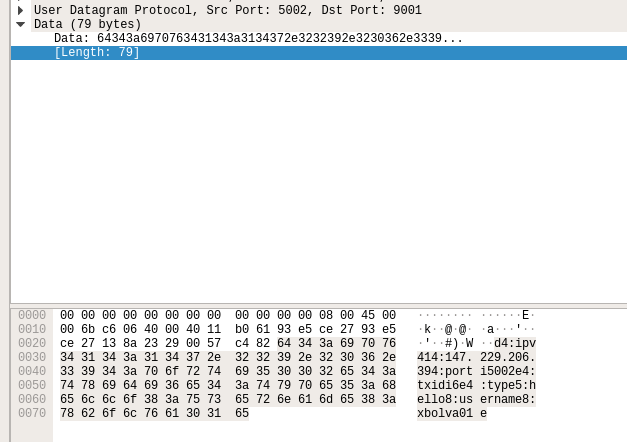
\includegraphics[width=\textwidth]{wireshark}
	\caption{Sledovanie Syslog správ vo Wiresharku}
\end{figure}


\chapter{Návod na použitie}

Program sa spúšťa cez terminál. Pri zadaní prepínača \textbf{-h/-{}-help} sa vypíše informačný text o~programe a jeho prepínačoch. V~prípade neznámeho či chybne použitého prepínača (nesprávna/chýbajúca hodnota prepínača) alebo pri akejkoľvek chybe v~sieťovej komunikácii sa program ukončí a o~probléme informuje používateľa správou na štandardný chybový výstup.

\begin{framed}
Použitie: isabot HOST[:PORT] CHANNELS [-s SYSLOG\_SERVER] [-l HIGHLIGHT] [-h|--help]

HOST je názov/IP adresa servera (napr. irc.freenode.net)

PORT je číslo portu (predvolené je 6667)

CHANNELS obsahuje jeden alebo viac kanálov (začínajú znakom \# alebo \&, oddelené sú čiarkou)

-s SYSLOG\_SERVER je IP adresa Syslog servera

-l HIGHLIGHT je zoznam kľúčových slov oddelených čiarkou (napr. ip,tcp,udp,isa)

-h|-{}-help zobrazenie informácii o~programe a o~prepínačoch
\end{framed}

Program sa ukončuje pomocou \textbf{Ctrl-C}, resp. pomocou príkazu \uv{\textbf{kill -INT <pid>}} v~termináli.


\chapter{Informácie o~programe}

Program sa skladá z~Makefile, ktorý slúži na zostavenie programu a nasledovných zdrojových súborov:

\begin{itemize}
\item isabot.cc
\item isabot.h
\item irc\_bot.cc
\item irc\_bot.h
\item irc\_command.cc
\item irc\_command.h
\item syslog\_server.cc
\item syslog\_server.h
\item utils.cc
\item utils.h
\end{itemize}

Spolu sa jedná o~813 riadkov zdrojového textu. Veľkosť výsledného binárneho súboru je 91,2 kB (preložené s~-02).

\chapter{Záver}
Projekt mal za cieľ vyskúšať si programovanie sieťovej služby. Bolo potrebné si naštudovať IRC a Syslog protokoly z~RFC dokumentov a následne tieto získané znalosti aplikovať v~implementácii samotného programu. Projekt overil nielen komplexne znalosti (analýza RFC dokumentov, práca s~BSD schránkami, programovanie v~C++, atď.) ale aj programatorské zručnosti - návrh, implementácia, ladenie a testovanie programu. Novozískané vedomosti z~tohto projektu sa týkali hlavne programovania sieťových aplikácií a protokolov (IRC, Syslog), na čo sú, čo umožňujú a ako fungujú.
